\documentclass[12pt]{article}
\usepackage{graphicx}
\usepackage{amsmath}
\begin{document}


\title{Exercises for Stochastic Linear Waves}
\date{November 10, 2016}
\author{Bendik Aleksander Sandvik\\}
\maketitle 
In this assignment we will do two exercises. The first one is about studying the buoy record of ocean waves in 1D. In the second we consider a temporal sequence.

\section{Exercise 1}

We've been given two files which we want to study:
\begin{itemize}
\item \verb|BayofBiscay.mat|
\item \verb|NewYearWave.mat|
\end{itemize}
As the first task, we want to plot the wave elevation as a time series. We do this by collecting the relevant parameters from the two files: 
\begin{itemize}
\item The time array $t$
\item The surface elevation $\eta$
\end{itemize}
We plot these parameters against each other to obtain the graphs given in figure 1 and figure 2.\\
Further on, we're asked to compute the significant wave height from the standard deviation of the data. We use the following relation:

$$ H_s^{BoB} \simeq 4 \sqrt{\sigma_{BoB}^2} = 2.61628 $$
$$ H_s^{NYW} \simeq 4 \sqrt{\sigma_{NYW}^2} = 11.9225 $$
\begin{figure}
  \caption{Data from the New Year Wave}
  \centering
    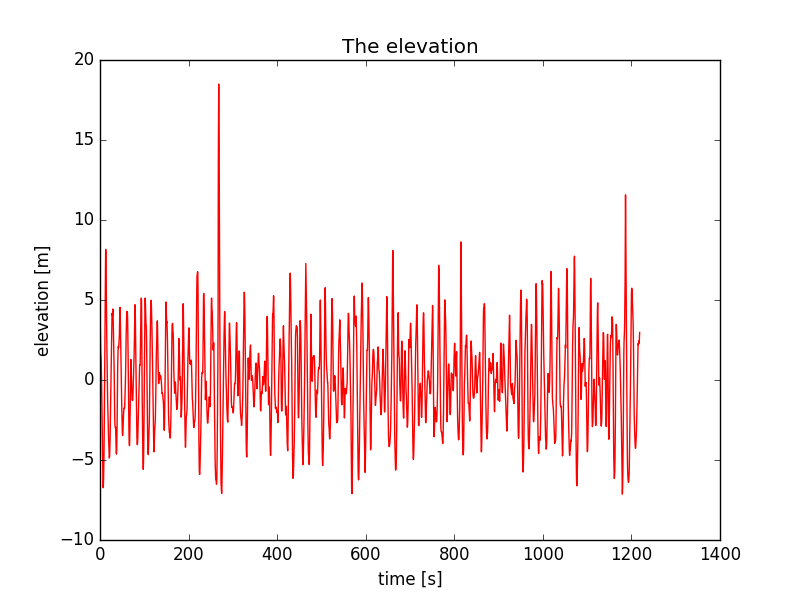
\includegraphics[width=0.5\textwidth]{NewYearWave.png}
\end{figure}
\begin{figure}
  \caption{Data from Beach of Biscay}
  \centering
    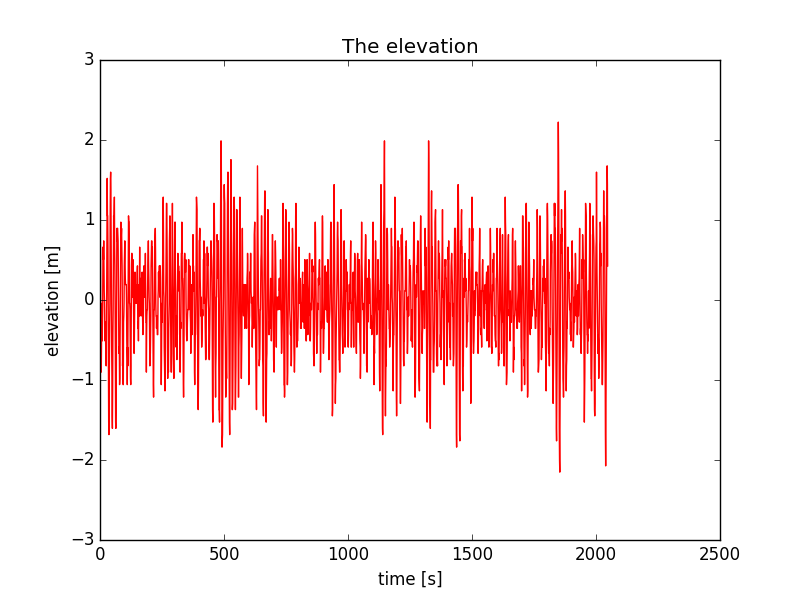
\includegraphics[width=0.5\textwidth]{BayOfBiscay.png}
\end{figure}
\begin{figure}
  \caption{Spectrum of the New Year Wave}
  \centering
    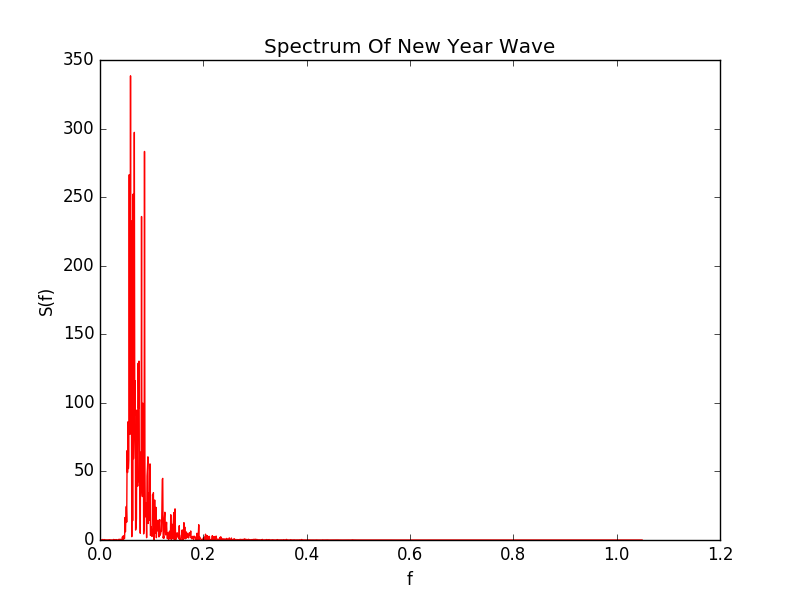
\includegraphics[width=0.5\textwidth]{SpectrumOfNewYearWave.png}
\end{figure}
\begin{figure}
  \caption{Spectrum of data from Beach of Biscay}
  \centering
    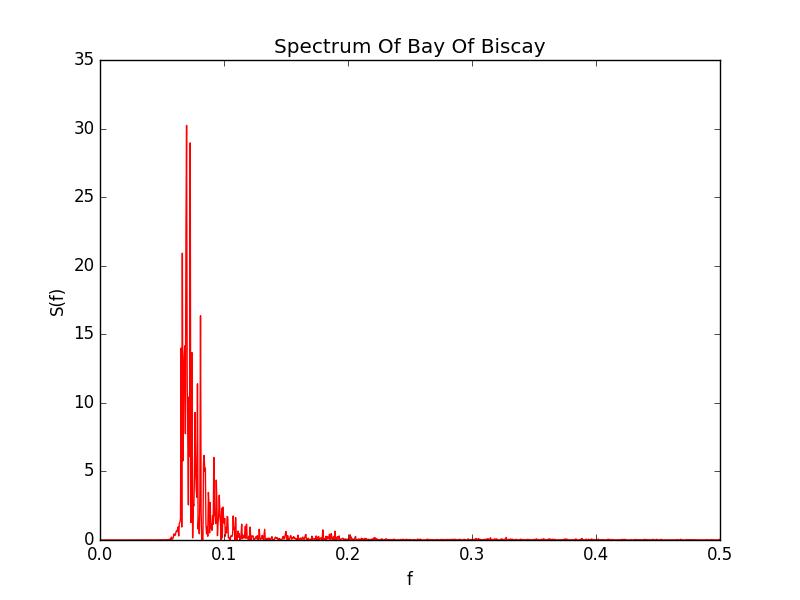
\includegraphics[width=0.5\textwidth]{SpectrumOfBayOfBiscay.png}
\end{figure} 
\\
To compute $\Delta f$ and the Nyquist limit, we use the following relations:
$$ \Delta f = \frac{1}{T}$$
$$ NQ_{limit} = \frac{1}{2 \Delta t}$$
Which is:
\\
\\
$ \Delta f_{BOB} = 0.000488281\;$   and $NQ_{limit} = 0.50$ for Beach of Biscay\\
$ \Delta f_{NYW} = 0.000820312$ and $NQ_{limit} = 1.05$ for New Year Wave\\
\\We're now interesting in estimation of the spectrum. We do this by:

$$\tilde{S}(f) = |\tilde{\eta}|^2 $$
where $\tilde{\eta}$ is the fourier-transform of the wave elevation, $\eta$. We find it for both files and obtain the graphs shown in figure 3 and figure 4.
\\
The spectral moments are given by:

$$ m_j = \int f^j S(f) df $$
But we estimate the moments by summation, instead of integration:
$$ m_j = \sum f^j S(f) df $$
Where we only consider positive frequencies. By this, we obtain the following moments:\\
\\
\\
$ m_0^{BOB} = 0.427803 \;$   and $m_0^{NYW} = 8.88408\;$\\
$ m_1^{BOB} = 0.0381729 \;$   and $m_1^{NYW} =0.72852\;$\\
$ m_2^{BOB} = 0.00448557\;$   and $m_1^{NYW} = 0.073303\;$\\
$ m_{-1}^{BOB} = 5.42263  \;$   and $m_{-1}^{NYW} =121.549\;$\\
\\
We use the zeroth-moment to compute the significant wave height:

$$ H_s^{BOB} \simeq 4 \sqrt{m_0^{BOB}} = 2.61628 $$
$$ H_s^{NYW} \simeq 4 \sqrt{m_0^{NYW}} = 11.9225 $$
We may also use the spectral moments to find the mean period estimations:

$$ T_{m01}^{BOB} = \frac{m_0^{BOB}}{m_1^{BOB}} = 11.207$$
$$ T_{m02}^{BOB} = \frac{m_1^{BOB}}{m_2^{BOB}} = 2.91722$$
$$ T_{m01}^{NYW} = \frac{m_0^{NYW}}{m_1^{NYW}} = 12.1947$$
$$ T_{m01}^{NYW} = \frac{m_1^{NYW}}{m_2^{NYW}} = 3.15254$$
We can't assume that S(f) describes the statistical behavior of all the individual waves in the record. The reason is shown by the new year wave. We get one really big wave, and several smaller ones. The values in the spectrum is given as a mean, which makes it impossible to predict if there are several medium waves, or several smaller waves with one, two or three really big waves. The bay of Biscay file gives an example of several medium waves.

\section{Exercise 2}

Now we want to study a 3D-case, which is given in the following files:
\begin{itemize}
\item \verb|Record3D_1.mat|
\item \verb|Record3D_2.mat|
\item \verb|Record3D_3.mat|
\end{itemize}
These gives us the following parameters:
\begin{itemize}
\item dt, sampling time $\Delta t$ in seconds
\item dx, sampling spatial in x-direction $Delta x$ in meters
\item dy, sampling spatial in y-direction $Delta y$ in meters
\item nx, steps in x-direction
\item ny, steps in y-direction
\item nt, steps in t
\item waves3d, Wave elevation field
\end{itemize}
We compute the spectral variables in the following way, and obtain the following result for the first file:\\\\
$\Delta k_x = \frac{2\pi}{L_x} = 0.00350624\;$ and $ NQ_x = \frac{1}{2 \Delta x} =  0.0714286$\\
$\Delta k_y = \frac{2\pi}{L_y} = 0.00350624\;$ and $ NQ_y = \frac{1}{2 \Delta y} = 0.0714286$\\
$\Delta w = \frac{2\pi}{T} = 0.0327249\;$ and $ NQ_t =\frac{1}{2 \Delta t}= 0.333333$\\\\
where $\;L_x = N_x \Delta x$, $\;L_y = N_y \Delta y$ and $\;T =  N_t \Delta t$.\\
As in exercise 1, we estimate the spectrum by considering:
$$\tilde{S}(f) = |\tilde{\eta}|^2 $$
where $\tilde{\eta}$ is the Fourier transform of $\eta(t,x,y)$. We plot this spectrum in three different cases:\\
1. w is constant, but bigger than $0.5$. This is figure 5.\\
2. $k_x = 0$. This is figure 6.\\
3. $k_y = 0$. This is figure 7.\\\\
By figure 6 and figure 7, we can see that the dispersion relation fits. The energy (the light area) is shaped just like the figure in the slide at page 35.\\\\ 
\\\\\\\\\\\
\begin{figure}
  \caption{Spectrum of Record3D 1.mat for w = constant}
  \centering
    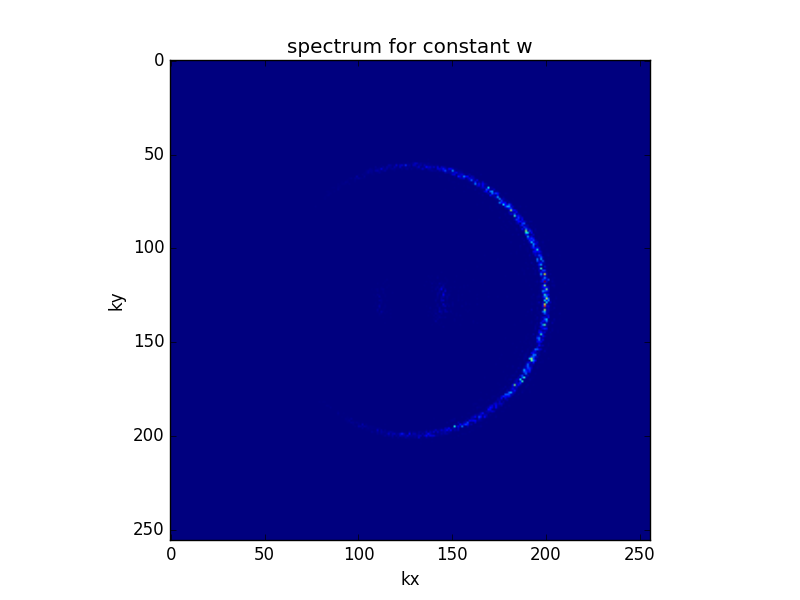
\includegraphics[width=0.5\textwidth]{spectrumW0.png}
\end{figure}

\begin{figure}
  \caption{Spectrum of Record3D 1.mat for kx = 0}
  \centering
    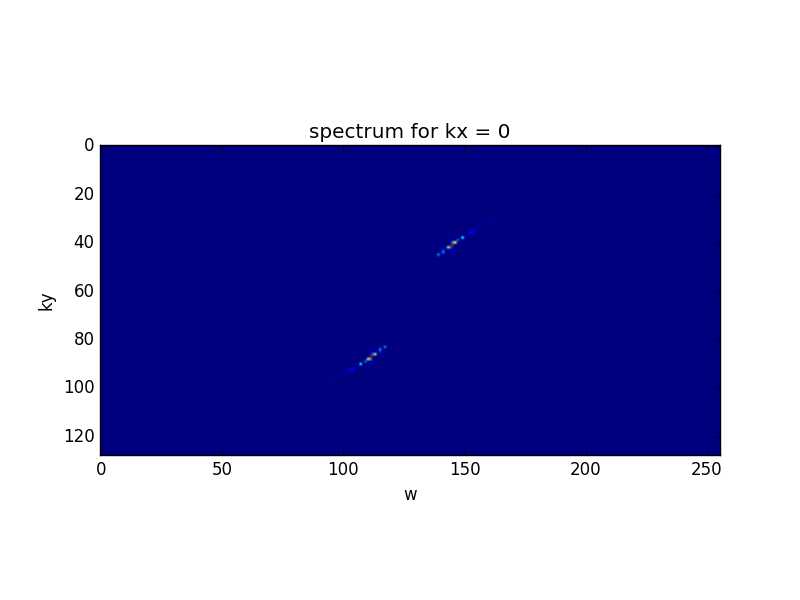
\includegraphics[width=0.5\textwidth]{spectrumkx=0.png}
\end{figure}

\begin{figure}
  \caption{Spectrum of Record3D 1.mat for ky = 0}
  \centering
    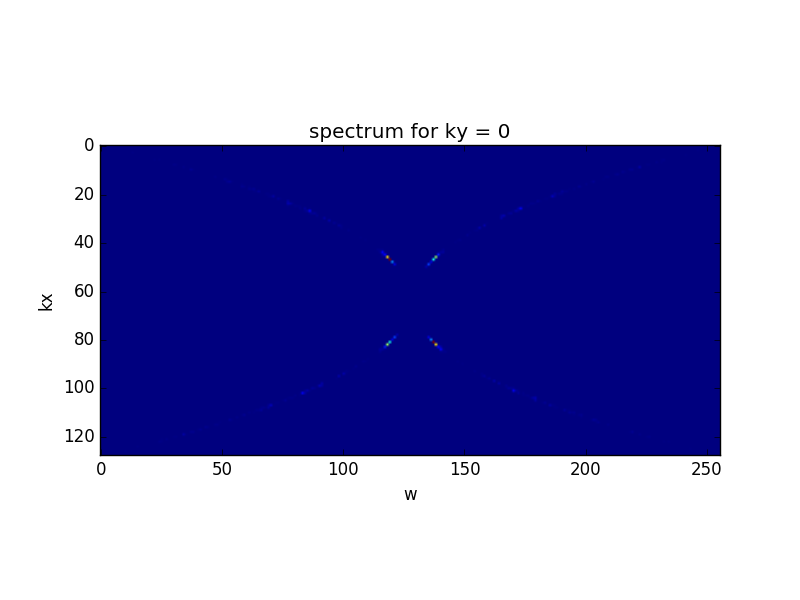
\includegraphics[width=0.5\textwidth]{spectrumky=0.png}
\end{figure}
Further on, we want to compute the unambiguous wave number spectrum, which we do by using the relation:

$$ F^{(2)}_+ = \int^{\infty}_0 F^{(3)}(\underline{k},w)dw $$

But since we do this in a discretized case, we estimate the unambiguous wave number spectrum by summation, instead of integration:
$$ F^{2}_+ = \sum F^{(3)}(\underline{k},w)dw$$
This is plotted in figure 8. \\Now we have three different ways to compute the significant wave height:\\
1. $H_s \simeq 4 \sigma = 4.53028$ computed from the standard deviation\\
2. $H_s = 4  m0 = 4.53028 \; $ computed from $F^{(3)}(\underline{k},w)$\\
3. $H_s \simeq 4 * \sigma = 2.56401$ computed from $F^{(2)}_{+}(\underline{k})$\\

Obviously is the 3rd alternative wrong. Unfortunately, I couldn't find the error. Please look at the file Read3D.py. The implimentation of this is at the end of the code. At last, we want to compare the three files. This is done by using the code Read3D.py and changing "FichData"-variable to the correct file we want to read. We expect the wind case to have the wides spectrum, the sweel to be more concentrated and the bimodal sea state to be the one with two uplighted areas.
The two other cases are plotted in figure 9 and figure 10.\\
1. Case 1 is the wind sea state\\
2. Case 2 is the bimodal sea state\\
3. Case 3 is the swell sea state\\



\begin{figure}
  \caption{Unambiguous wave number spectrum for case 1}
  \centering
    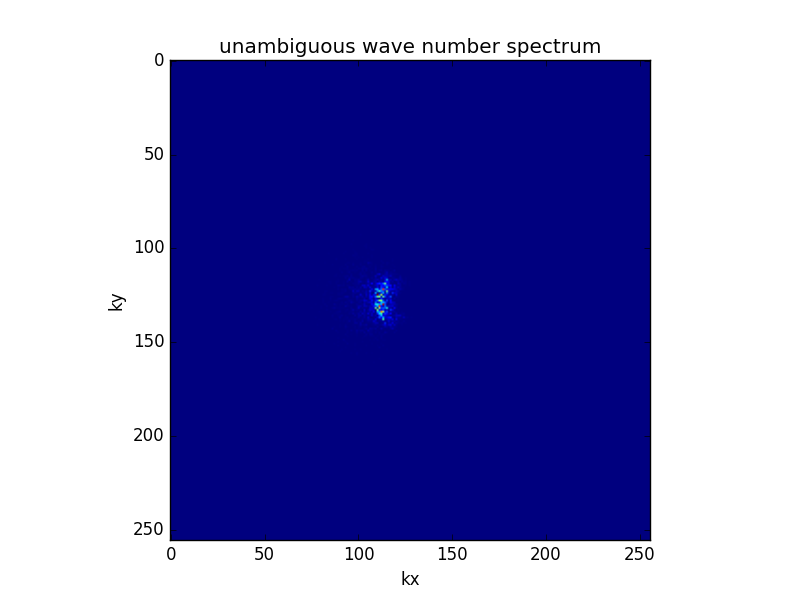
\includegraphics[width=0.5\textwidth]{unam_w_n_s.png}
\end{figure}

\begin{figure}
  \caption{Unambiguous wave number spectrum for case 2}
  \centering
    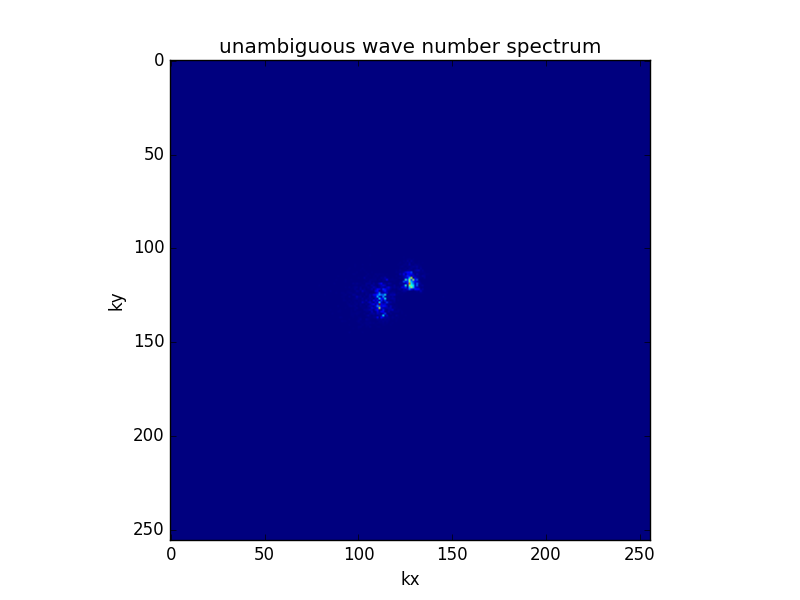
\includegraphics[width=0.5\textwidth]{unam_w_n_s_2.png}
\end{figure}

\begin{figure}
  \caption{Unambiguous wave number spectrum for case 3}
  \centering
    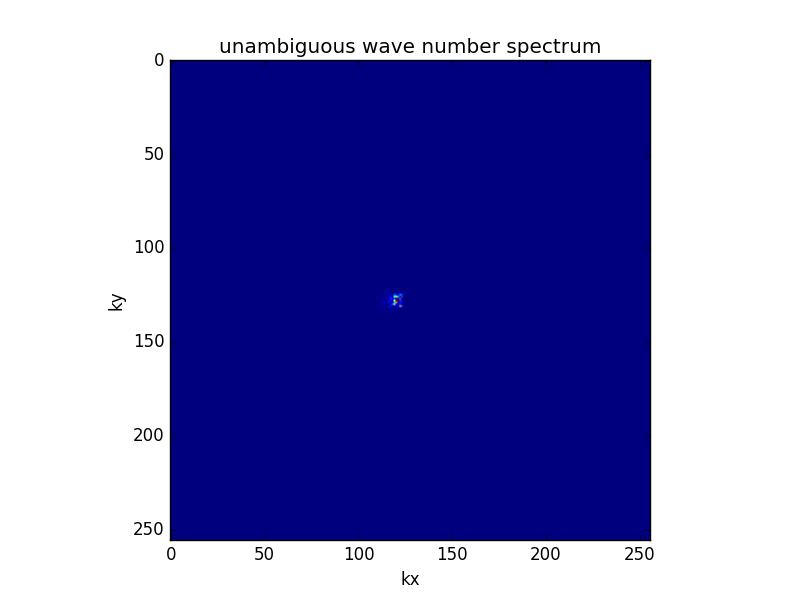
\includegraphics[width=0.5\textwidth]{unam_w_n_s_3.png}
\end{figure}


\end{document}